%!TEX root = main.tex
\vspace{-15pt}
\section{Fixing Boundary Imperfections\label{precision}}%: Aggregation v.s. Retrieval Comparison}
% \subsection{Retrieval-based methods}
% This class of algorithms tries to identify good and bad workers, and then chooses the best worker segmentation as the output segmentation. In this paper, we look at two different ways of ranking workers and choosing the best worker. First, we use the {\em number of control points}, i.e. number of vertices in a worker's segmentation polygon to rank workers. This is a ranking scheme that~\cite{Vittayakorn2011} showed performs well in practice. Intuitively, workers that have used a larger number of points are likely to have been more precise, and provided a more complex and accurate segmentation. Other heuristic ranking scheme is described in more detail in our technical report~\cite{segmentation-tr}.
% \begin{figure}[h!]
% \vspace{-10pt}
% \centering
% 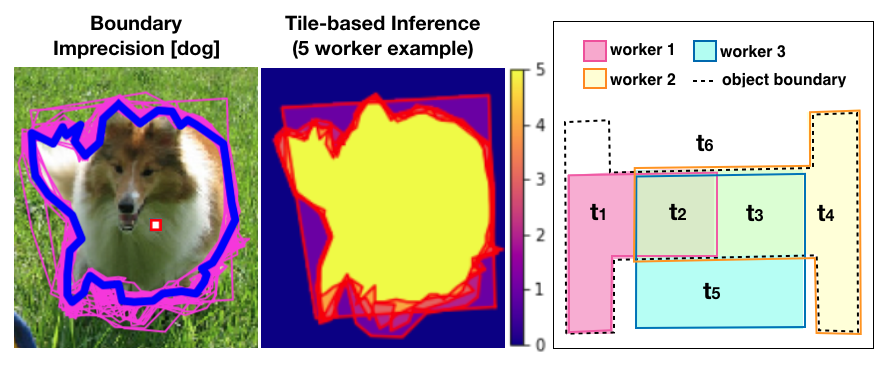
\includegraphics[width=0.8\textwidth]{plots/precision_issue_tile_example.png}
% \caption{Left: Pink boundaries shows worker segmentations and blue delineates the ground truth. Right: Segmentation boundaries drawn by five workers shown in red. Overlaid segmentation creates a masks where the color indicates the number of workers who voted for the tile region.}
% \label{tile_demo}
% \end{figure}
% \vspace{-10pt}

% , where we logically overlay all workers' segmentations on top of each other, as illustrated in Figure \ref{tile_demo} right, to create non-overlapping discrete tile units. 
At the heart of our aggregation techniques is the \emph{tile data representation}. A tile is the smallest non-overlapping discrete unit created by overlaying all of the workers' segmentations on top of each other. %with a certain probability of being contained in the ground truth segmentation. 
The tile representation allows us to aggregate segmentations from multiple workers, rather than being restricted to a single worker's segmentation---allowing us to fix one worker's errors with help from another. \changes{In Figure \ref{tile_demo} (right), we display three worker segmentations for a toy example with 6 resulting tiles. Any subset of these tiles can contribute towards the final segmentation.}
%both worker 1 and 2's segmentation can contribute towards the final segmentation.
\par This simple but powerful idea of tiles also allows us to reformulate our problem from one of ``generating a segmentation'' to a setting that is much more familiar to crowdsourcing researchers. Since tiles are the lowest granularity units created by overlaying all workers' segmentations on top of each other, each tile is either completely contained within or outside a given worker segmentation. Specifically, we can regard a worker segmentation as multiple boolean responses where they have voted `yes' or `no' to every tile independently. Intuitively, a worker votes `yes' for every tile that is contained in their segmentation, and `no' for every tile that is not. As shown in Figure \ref{tile_demo} (right), tile $t_2$ is voted `yes' by worker 1, 2, and 3; tile $t_3$ is voted `yes' by worker 2 and 3. The goal of our aggregation algorithms is to pick an appropriate set of tiles that effectively trades off precision versus recall.
%\par Now, our problem of choosing a set of tiles to form a segmentation boils down to aggregating multiple boolean responses on every individual tile. Tiles with a final aggregated answer of ``yes'' are included in our output segmentation, while the remaining tiles are excluded. We should note that tiles need not necessarily be completely contained or completely outside the ground truth segmentation, therefore not every tile has a ground truth boolean answer. For tiles that are not completely contained or completely excluded in the ground truth, we gain recall but lose precision if we include them in our output segmentation, or lose recall and gain precision if we don't include them in our output segmentation. The goal of our aggregation algorithms, described below, is to pick a good set of tiles that effectively trade-off precision versus recall.
% The intuition here is that by splitting the image into tiles, we get finer granularity information than by looking at complete segmentations. This also allows us to aggregate data from multiple workers rather than having to choose a single worker bounding box---enabling the opportunity to choose partial segmentations by fixing one worker's errors via the help from another worker's segmentation.
% Now, we will describe several algorithms for picking a good set of tiles.
%The goal of our aggregation algorithms, described below, is to pick a good set of tiles that effectively trade-off precision versus recall.
\par Now that we have modeled segmentation as a collection of worker votes for tiles, we can now develop familiar variants of standard quality evaluation algorithms for this setting.

\stitle{Aggregation: Majority Vote Aggregation (MV)} 
\par \noindent This simple algorithm includes a tile in the output segmentation if and only if the tile has `yes' votes from at least 50\% of all worker segmentations.

\stitle{Aggregation: Expectation-Maximization (EM)}
\par \noindent Unlike MV, which assumes that all workers perform uniformly, EM approaches use worker quality models to infer the likelihood that a tile is part of the ground truth segmentation. While simultaneously estimating worker qualities and tile likelihoods as hidden variables, 
%The EM algorithm simultaneously estimates both worker qualities and tile likelihoods as hidden variables. 
our basic worker quality model that we evaluate in Section~\ref{sec:experiment} assumes a fixed probability for a correct vote.
%is based on the probability that the worker will vote for a tile correctly. 
\techreport{Another model variant accounts for tile areas based on the intuition that workers should be penalized more if they make a mistake on a large tile (e.g. yellow tile in Figure \ref{tile_demo} middle) than on a small tile (e.g. orange tiles near the boundary in Figure \ref{tile_demo} middle). Our advanced %4-parameter Bernoulli 
worker quality model additionally accounts for true- and false-positive rates of the worker's tile votes.}Details of the formal derivation and other more fine-grained worker quality models can be found in our technical report.
%\agp{if we don't evaluate all of these we should drop these description. Also, cite the algo we are adopting in Sec 6.}

\stitle{Aggregation: Greedy Tile Picking (greedy)} 
%, and then picks tiles in that order, effectively picking tiles in order of their contribution to the Jaccard similarity against ground truth, 
\par \noindent The greedy algorithm picks tiles in descending order based on the ratios of overlap area to non-overlap area (both with respect to ground truth), for as long as the estimated Jaccard similarity of the resulting segmentation continue to increase. Since the tile overlap and non-overlap against ground truth are unknown, we use tile-inclusion probabilities from EM to estimate these areas as a heuristic. Furthermore, since we cannot compute the actual Jaccard similarity against the unknown ground truth, we use a heuristic baseline such as MV as a proxy for the ground truth. Intuitively, tiles that have a high overlap area and low non-overlap area contribute to high recall, at the cost of relatively little precision error. We include a proof in our technical report showing that picking tiles in such an order maximizes the Jaccard similarity of the resulting segmentation locally at every step. 

\stitle{Retrieval: Number of Control Points (num pts)}
\par \noindent This algorithm picks the worker segmentation with the largest number of control points around the segmentation boundary (i.e., the most precise drawing) as the output segmentation \cite{Vittayakorn2011,Sorokin2008}.

\begin{figure}[h!]
\centering
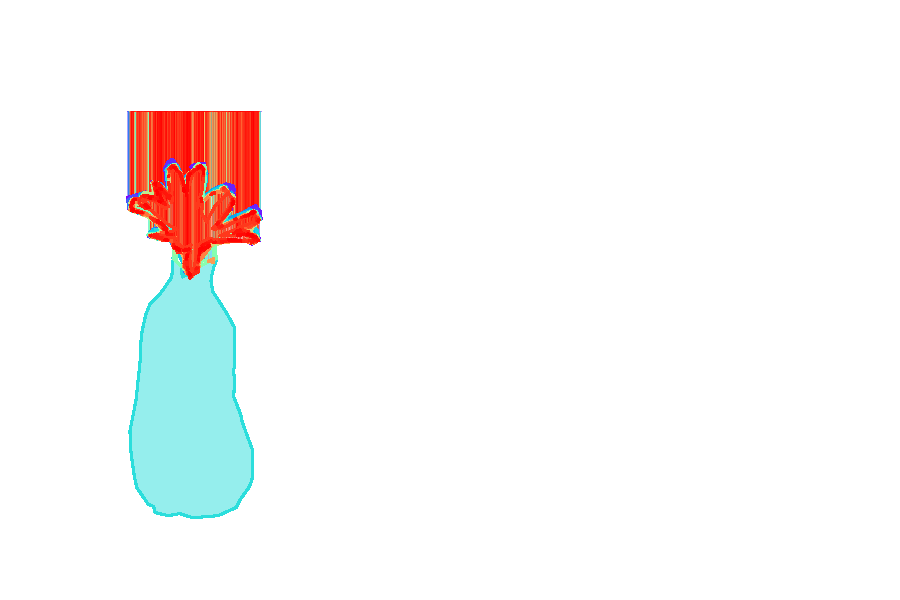
\includegraphics[width=0.85\linewidth]{plots/tile.pdf}
\caption{Left: Toy example demonstrating tiles created by three workers' segmentations around an object delineated by the black dotted line. Right: Segmentation boundaries drawn by five workers shown in red. Overlaid segmentation creates a mask where the color indicates the number of workers who voted for the tile region.}
\label{tile_demo}
\setlength{\abovecaptionskip}{-15pt}
\setlength{\belowcaptionskip}{-25pt}
\end{figure}  